\clearpage
\section{Discussion and Limitations}\label{sec:discussion}

The results show that the performance gains achieved using SSL are not always significant
(Table~\ref{tab:ssl-overview}). With 1,000 labels, the best semi-supervised method beats the
Optuna-tuned supervised baseline by at most \MagInImpr\% (magnetism, Self-Training). On
metallicity and stability the gain is within one standard deviation, and with the GNoME pool
on metallicity no SSL method beats the baseline at all. This suggests that SSL is not a
universal solution and that its effectiveness depends on data distribution and underlying
assumptions:
\begin{itemize}
  \item \textbf{Strong baselines.} Gradient-boosted trees trained on 142 Magpie descriptors
  already capture most of what 1,000 labels can teach. The label-budget curves show that SSL
  helps most at 250--500 labels and that the gap closes after 2,500 labels.
  \item \textbf{Distribution shift.} The KS statistics between labeled and GNoME compositions
  reach 0.48 (Figure~\ref{fig:shift}). Unlabeled data from a different distribution violate the
  cluster and manifold assumptions, which is why the GNoME pool is never better than the
  same-database pool for the graph methods.
  \item \textbf{More unlabeled data is not better.} For almost every method the composite
  score decreases from 1,000 to 100,000 unlabeled compositions: errors in the pseudo-labels
  accumulate faster than useful information. Only Self-Training with a high confidence
  threshold (0.9) is robust to the pool size.
  \item \textbf{Graph methods do not scale to this feature space.} Label Propagation and
  Label Spreading are always last, even after class-mass normalization. Euclidean neighbours in
  descriptor space do not share labels reliably, and an exact RBF graph is only possible for
  the smallest pools.
  \item \textbf{Composition-only descriptors.} Stability (\StabSelComp{} composite even after
  deployment) depends on the crystal structure and on competing phases, which a composition
  cannot encode. Structure-aware graph neural networks (CGCNN, MEGNet, ALIGNN) would be needed
  for a large gain.
  \item \textbf{DFT labels.} All labels come from PBE calculations. PBE underestimates band
  gaps by 30--50\% on average, so the 1.1--1.7\,eV photovoltaic window is a window on
  \emph{PBE} gaps, and real absorbers may fall slightly outside it.
\end{itemize}

The self-supervised masked autoencoder learns a good representation (R$^2$ = \AERtwo{} on all
descriptors, \AERtwoMasked{} on the hidden ones). As extra features it is tied with the raw
descriptors on metallicity and slightly below them on magnetism and stability, but it gives a compact 32-dimensional space for the nearest-material search of
the application. The unsupervised analysis (Apriori rules, K-Means) gives interpretable
chemistry, for example \{Fe\} $\Rightarrow$ MAGNETIC with a lift of 3.4, and helps explain the
models, but it does not replace a classifier.

The traditional materials-informatics approach for the photovoltaic band gap demonstrated
that, for a well-defined target, classical methods with feature optimization provide strong
performance with interpretability. The genetic algorithm successfully identified \GAFinalN{}
key descriptors from an initial set of 142 (a 63\% reduction) with a test ROC-AUC of
\GapGAAUC{} against \GapAllAUC{} for all descriptors, and the applicability domain covers
\ADFracIn\% of the test compositions.

Alternative approaches such as Active Learning, Transfer Learning, or deep representations of
materials may provide better results in certain scenarios. Since our models are cheap to
evaluate and the GNoME pool is huge, the most promising next step is a semi-supervised
\emph{active-learning} loop (Figure~\ref{fig:al}): instead of labelling random compositions,
the model chooses the most informative or most promising candidates, these are computed by
DFT, and the model is re-trained.

\begin{figure}[H]
  \centering
  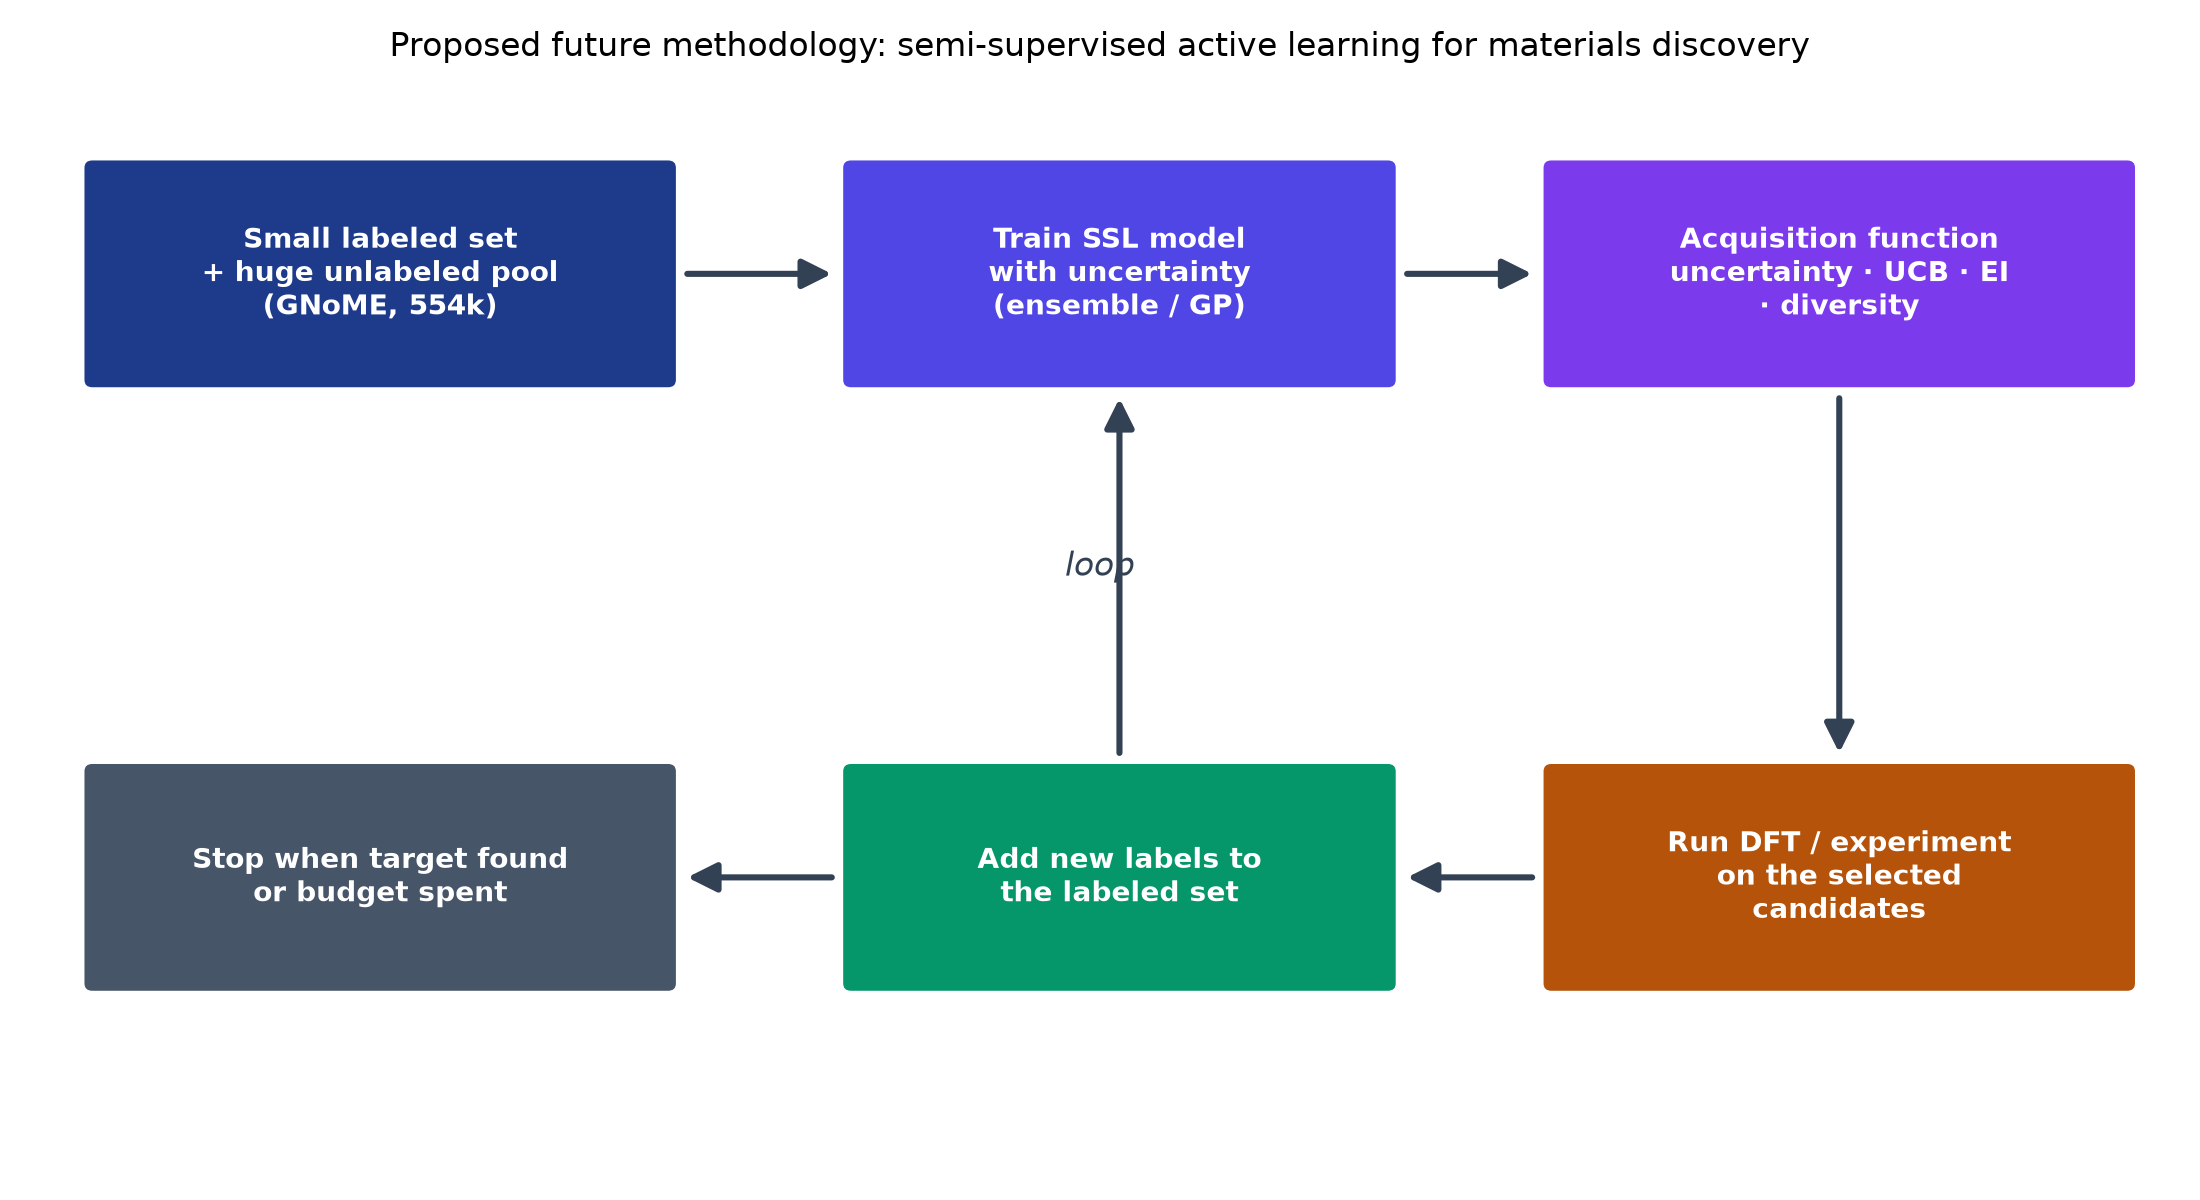
\includegraphics[width=\textwidth]{schematics/active_learning_loop.png}
  \caption{Better methodology for future: semi-supervised active learning.}\label{fig:al}
\end{figure}
